% Options for packages loaded elsewhere
\PassOptionsToPackage{unicode}{hyperref}
\PassOptionsToPackage{hyphens}{url}
\PassOptionsToPackage{dvipsnames,svgnames*,x11names*}{xcolor}
%
\documentclass[
]{article}
\usepackage{amsmath,amssymb}
\usepackage{lmodern}
\usepackage{ifxetex,ifluatex}
\ifnum 0\ifxetex 1\fi\ifluatex 1\fi=0 % if pdftex
  \usepackage[T1]{fontenc}
  \usepackage[utf8]{inputenc}
  \usepackage{textcomp} % provide euro and other symbols
\else % if luatex or xetex
  \usepackage{unicode-math}
  \defaultfontfeatures{Scale=MatchLowercase}
  \defaultfontfeatures[\rmfamily]{Ligatures=TeX,Scale=1}
\fi
% Use upquote if available, for straight quotes in verbatim environments
\IfFileExists{upquote.sty}{\usepackage{upquote}}{}
\IfFileExists{microtype.sty}{% use microtype if available
  \usepackage[]{microtype}
  \UseMicrotypeSet[protrusion]{basicmath} % disable protrusion for tt fonts
}{}
\makeatletter
\@ifundefined{KOMAClassName}{% if non-KOMA class
  \IfFileExists{parskip.sty}{%
    \usepackage{parskip}
  }{% else
    \setlength{\parindent}{0pt}
    \setlength{\parskip}{6pt plus 2pt minus 1pt}}
}{% if KOMA class
  \KOMAoptions{parskip=half}}
\makeatother
\usepackage{xcolor}
\IfFileExists{xurl.sty}{\usepackage{xurl}}{} % add URL line breaks if available
\IfFileExists{bookmark.sty}{\usepackage{bookmark}}{\usepackage{hyperref}}
\hypersetup{
  pdftitle={Log of Crab body metrics - predicting the subspecies of crabs},
  pdfauthor={IJsbrand Pool, 403589},
  colorlinks=true,
  linkcolor=blue,
  filecolor=Maroon,
  citecolor=Blue,
  urlcolor=Blue,
  pdfcreator={LaTeX via pandoc}}
\urlstyle{same} % disable monospaced font for URLs
\usepackage[margin=1in]{geometry}
\usepackage{color}
\usepackage{fancyvrb}
\newcommand{\VerbBar}{|}
\newcommand{\VERB}{\Verb[commandchars=\\\{\}]}
\DefineVerbatimEnvironment{Highlighting}{Verbatim}{commandchars=\\\{\}}
% Add ',fontsize=\small' for more characters per line
\newenvironment{Shaded}{}{}
\newcommand{\AlertTok}[1]{\textcolor[rgb]{1.00,0.00,0.00}{#1}}
\newcommand{\AnnotationTok}[1]{\textcolor[rgb]{0.00,0.50,0.00}{#1}}
\newcommand{\AttributeTok}[1]{#1}
\newcommand{\BaseNTok}[1]{#1}
\newcommand{\BuiltInTok}[1]{#1}
\newcommand{\CharTok}[1]{\textcolor[rgb]{0.00,0.50,0.50}{#1}}
\newcommand{\CommentTok}[1]{\textcolor[rgb]{0.00,0.50,0.00}{#1}}
\newcommand{\CommentVarTok}[1]{\textcolor[rgb]{0.00,0.50,0.00}{#1}}
\newcommand{\ConstantTok}[1]{#1}
\newcommand{\ControlFlowTok}[1]{\textcolor[rgb]{0.00,0.00,1.00}{#1}}
\newcommand{\DataTypeTok}[1]{#1}
\newcommand{\DecValTok}[1]{#1}
\newcommand{\DocumentationTok}[1]{\textcolor[rgb]{0.00,0.50,0.00}{#1}}
\newcommand{\ErrorTok}[1]{\textcolor[rgb]{1.00,0.00,0.00}{\textbf{#1}}}
\newcommand{\ExtensionTok}[1]{#1}
\newcommand{\FloatTok}[1]{#1}
\newcommand{\FunctionTok}[1]{#1}
\newcommand{\ImportTok}[1]{#1}
\newcommand{\InformationTok}[1]{\textcolor[rgb]{0.00,0.50,0.00}{#1}}
\newcommand{\KeywordTok}[1]{\textcolor[rgb]{0.00,0.00,1.00}{#1}}
\newcommand{\NormalTok}[1]{#1}
\newcommand{\OperatorTok}[1]{#1}
\newcommand{\OtherTok}[1]{\textcolor[rgb]{1.00,0.25,0.00}{#1}}
\newcommand{\PreprocessorTok}[1]{\textcolor[rgb]{1.00,0.25,0.00}{#1}}
\newcommand{\RegionMarkerTok}[1]{#1}
\newcommand{\SpecialCharTok}[1]{\textcolor[rgb]{0.00,0.50,0.50}{#1}}
\newcommand{\SpecialStringTok}[1]{\textcolor[rgb]{0.00,0.50,0.50}{#1}}
\newcommand{\StringTok}[1]{\textcolor[rgb]{0.00,0.50,0.50}{#1}}
\newcommand{\VariableTok}[1]{#1}
\newcommand{\VerbatimStringTok}[1]{\textcolor[rgb]{0.00,0.50,0.50}{#1}}
\newcommand{\WarningTok}[1]{\textcolor[rgb]{0.00,0.50,0.00}{\textbf{#1}}}
\usepackage{graphicx}
\makeatletter
\def\maxwidth{\ifdim\Gin@nat@width>\linewidth\linewidth\else\Gin@nat@width\fi}
\def\maxheight{\ifdim\Gin@nat@height>\textheight\textheight\else\Gin@nat@height\fi}
\makeatother
% Scale images if necessary, so that they will not overflow the page
% margins by default, and it is still possible to overwrite the defaults
% using explicit options in \includegraphics[width, height, ...]{}
\setkeys{Gin}{width=\maxwidth,height=\maxheight,keepaspectratio}
% Set default figure placement to htbp
\makeatletter
\def\fps@figure{htbp}
\makeatother
\setlength{\emergencystretch}{3em} % prevent overfull lines
\providecommand{\tightlist}{%
  \setlength{\itemsep}{0pt}\setlength{\parskip}{0pt}}
\setcounter{secnumdepth}{5}
\usepackage{graphicx}
\usepackage{float}
\usepackage{booktabs}
\usepackage{longtable}
\usepackage{array}
\usepackage{multirow}
\usepackage{wrapfig}
\usepackage{float}
\usepackage{colortbl}
\usepackage{pdflscape}
\usepackage{tabu}
\usepackage{threeparttable}
\usepackage{threeparttablex}
\usepackage[normalem]{ulem}
\usepackage{makecell}
\usepackage{xcolor}
\ifluatex
  \usepackage{selnolig}  % disable illegal ligatures
\fi

\title{Log of Crab body metrics - predicting the subspecies of crabs}
\author{IJsbrand Pool, 403589}
\date{}

\begin{document}
\maketitle

{
\hypersetup{linkcolor=}
\setcounter{tocdepth}{2}
\tableofcontents
}
\newpage

\hypertarget{logbook-eda}{%
\section{Logbook EDA}\label{logbook-eda}}

\hypertarget{dataset-information}{%
\subsection{Dataset information}\label{dataset-information}}

The rock crab \emph{Leptograpsus variegatus}, is recorded as occurring
on a number of southern Pacific islands, the western coast of South
America, and the coasts of Australia south of the Tropic of Capricorn.
Mahon, using ecological studies which extended those of Shield, and a
genetical analysis based on an electrophoretic study, established the
specific distinctness of rock crabs of the blue and orange forms of the
genus \emph{Leptograpsus} which occur on the coasts of Australia. These
colour forms were previously regarded as morphs of \emph{L. variegatus.}

In an attempt to resolve this problem of identification, a morphological
study of the Western Australian species was undertaken. This paper
reports an exploratory data analysis of the data and a machine learning
algorithm to predict the species of the crab based on this data.

The dataset used is the crab body metrics dataset by Campbell, N.A. and
Mahon, R.J. (1974) A multivariate study of variation in two species of
rock crab of genus \emph{Leptograpsus}{[}1{]}. This data set contains
multiple morphological metrics of the bodies of \emph{L. variegatus.}
crabs, and the gender and color of the crab. The measured metrics are
the frontal lobe size, rear width, carapace length, carapace width and
body depth. All these values are in millimeters. There are 100 orange
and 100 blue crabs. 50 crabs of each gender per color of crab.

\hypertarget{research-question}{%
\subsubsection{Research question}\label{research-question}}

The goal of this project was to find out if the subspecies of a
\emph{Leptograpsus variegatus} was predictable.To find out if this is
possible, a research question had to be formulated. The research
question for this project is ``Can the species of a \emph{L.variegatus}
be determined based on some morphological measurements of its
carapace''. To answer this question, the data was first explored and
cleaned. Then, multiple machine learning algorithms were tested to find
what algorithm could be used best.

\newpage

\hypertarget{data-analysis}{%
\subsection{Data analysis}\label{data-analysis}}

\begin{Shaded}
\begin{Highlighting}[]
\CommentTok{\#load in the data}
\NormalTok{myData }\OtherTok{\textless{}{-}} \FunctionTok{read.csv}\NormalTok{(}\StringTok{"datafiles/data.csv"}\NormalTok{)}
\end{Highlighting}
\end{Shaded}

After the data was loaded in, a codebook with the attribute names and
their descriptions was generated, shown in table 2. To get a better view
of the measurements in the dataset, a five number summary was created
for each attribute. These values are shown in table 3. The table shows
that the mean and the median are close in value for each column, meaning
that they all are normal distributions.

\begin{Shaded}
\begin{Highlighting}[]
\CommentTok{\#create the codebook}
\NormalTok{column }\OtherTok{\textless{}{-}} \FunctionTok{colnames}\NormalTok{(myData)}
\NormalTok{description }\OtherTok{\textless{}{-}} \FunctionTok{c}\NormalTok{(}\StringTok{"Species"}\NormalTok{, }\StringTok{"Sex"}\NormalTok{, }\StringTok{"Index"}\NormalTok{, }\StringTok{"Frontal lobe size (mm)"}\NormalTok{, }\StringTok{"Rear width (mm)"}\NormalTok{, }\StringTok{"Carapace length (mm)"}\NormalTok{, }\StringTok{"Carapace width (mm)"}\NormalTok{, }\StringTok{"Body depth (mm)"}\NormalTok{)}
\NormalTok{codebook }\OtherTok{\textless{}{-}} \FunctionTok{data.frame}\NormalTok{(column, description)}
\FunctionTok{kable}\NormalTok{(codebook, }\AttributeTok{caption =} \StringTok{"Codebook of the dataset"}\NormalTok{) }\SpecialCharTok{\%\textgreater{}\%} 
\FunctionTok{kable\_styling}\NormalTok{(}\AttributeTok{font\_size =} \DecValTok{10}\NormalTok{, }\AttributeTok{latex\_options =} \StringTok{"hold\_position"}\NormalTok{)}
\end{Highlighting}
\end{Shaded}

\begin{table}[!h]

\caption{\label{tab:codebook}Codebook of the dataset}
\centering
\fontsize{10}{12}\selectfont
\begin{tabular}[t]{l|l}
\hline
column & description\\
\hline
sp & Species\\
\hline
sex & Sex\\
\hline
index & Index\\
\hline
FL & Frontal lobe size (mm)\\
\hline
RW & Rear width (mm)\\
\hline
CL & Carapace length (mm)\\
\hline
CW & Carapace width (mm)\\
\hline
BD & Body depth (mm)\\
\hline
\end{tabular}
\end{table}

\begin{Shaded}
\begin{Highlighting}[]
\NormalTok{sumdat }\OtherTok{\textless{}{-}} \FunctionTok{summary}\NormalTok{(myData[}\DecValTok{4}\SpecialCharTok{:}\DecValTok{8}\NormalTok{])}
\NormalTok{sumdat }\OtherTok{\textless{}{-}} \FunctionTok{sub}\NormalTok{(}\StringTok{".*:"}\NormalTok{, }\StringTok{""}\NormalTok{, sumdat)}
\FunctionTok{rownames}\NormalTok{(sumdat) }\OtherTok{\textless{}{-}}  \FunctionTok{c}\NormalTok{(}\StringTok{"Minimum"}\NormalTok{, }\StringTok{"Q1"}\NormalTok{, }\StringTok{"Median"}\NormalTok{, }\StringTok{"Mean"}\NormalTok{, }\StringTok{"Q3"}\NormalTok{, }\StringTok{"Maximum"}\NormalTok{)}
\FunctionTok{colnames}\NormalTok{(sumdat) }\OtherTok{\textless{}{-}} \FunctionTok{c}\NormalTok{(}\StringTok{"Frontal Lobe"}\NormalTok{, }\StringTok{"Rear Width"}\NormalTok{, }\StringTok{"Carapace Length"}\NormalTok{, }\StringTok{"Carapace Width"}\NormalTok{, }\StringTok{"Body Depth"}\NormalTok{)}
\FunctionTok{kable}\NormalTok{(sumdat, }\AttributeTok{caption =} \StringTok{"Five number summary of the morphological measurements of the crab bodies."}\NormalTok{) }\SpecialCharTok{\%\textgreater{}\%} 
\FunctionTok{kable\_styling}\NormalTok{(}\AttributeTok{latex\_options =} \StringTok{"hold\_position"}\NormalTok{)}
\end{Highlighting}
\end{Shaded}

\begin{table}[!h]

\caption{\label{tab:summary}Five number summary of the morphological measurements of the crab bodies.}
\centering
\begin{tabular}[t]{l|l|l|l|l|l}
\hline
  & Frontal Lobe & Rear Width & Carapace Length & Carapace Width & Body Depth\\
\hline
Minimum & 7.20 & 6.50 & 14.70 & 17.10 & 6.10\\
\hline
Q1 & 12.90 & 11.00 & 27.27 & 31.50 & 11.40\\
\hline
Median & 15.55 & 12.80 & 32.10 & 36.80 & 13.90\\
\hline
Mean & 15.58 & 12.74 & 32.11 & 36.41 & 14.03\\
\hline
Q3 & 18.05 & 14.30 & 37.23 & 42.00 & 16.60\\
\hline
Maximum & 23.10 & 20.20 & 47.60 & 54.60 & 21.60\\
\hline
\end{tabular}
\end{table}

\newpage

\hypertarget{visualisation}{%
\subsection{Visualisation}\label{visualisation}}

\hypertarget{scatterplot-for-frontal-lobe-size-against-carapace-width}{%
\subsubsection{Scatterplot for frontal lobe size against carapace
width}\label{scatterplot-for-frontal-lobe-size-against-carapace-width}}

\begin{Shaded}
\begin{Highlighting}[]
\CommentTok{\#plot the Front lobe size against Carapace width}
\FunctionTok{ggplot}\NormalTok{() }\SpecialCharTok{+}
  \FunctionTok{geom\_point}\NormalTok{(}\AttributeTok{data =}\NormalTok{ myData[myData}\SpecialCharTok{$}\NormalTok{sp }\SpecialCharTok{==} \StringTok{"B"}\NormalTok{,], }\AttributeTok{mapping =} \FunctionTok{aes}\NormalTok{(}\AttributeTok{x =}\NormalTok{ FL, }\AttributeTok{y =}\NormalTok{ CW, }\AttributeTok{color =} \StringTok{\textquotesingle{}Blue\textquotesingle{}}\NormalTok{)) }\SpecialCharTok{+}
  \FunctionTok{geom\_point}\NormalTok{(}\AttributeTok{data =}\NormalTok{ myData[myData}\SpecialCharTok{$}\NormalTok{sp }\SpecialCharTok{==} \StringTok{"O"}\NormalTok{,], }\AttributeTok{mapping =} \FunctionTok{aes}\NormalTok{(}\AttributeTok{x =}\NormalTok{ FL, }\AttributeTok{y =}\NormalTok{ CW, }\AttributeTok{color =} \StringTok{\textquotesingle{}Orange\textquotesingle{}}\NormalTok{)) }\SpecialCharTok{+}
  \FunctionTok{scale\_color\_manual}\NormalTok{(}\AttributeTok{values=}\FunctionTok{c}\NormalTok{(}\StringTok{"\#4444EE"}\NormalTok{, }\StringTok{"\#E69F00"}\NormalTok{)) }\SpecialCharTok{+}
  \FunctionTok{labs}\NormalTok{(}\AttributeTok{x =} \StringTok{"Frontal lobe size (mm)"}\NormalTok{, }\AttributeTok{y =} \StringTok{"Carapace width (mm)"}\NormalTok{, }\AttributeTok{title=}\StringTok{\textquotesingle{}Front lobe size against Carapace width\textquotesingle{}}\NormalTok{)}
\end{Highlighting}
\end{Shaded}

\begin{figure}[H]

{\centering 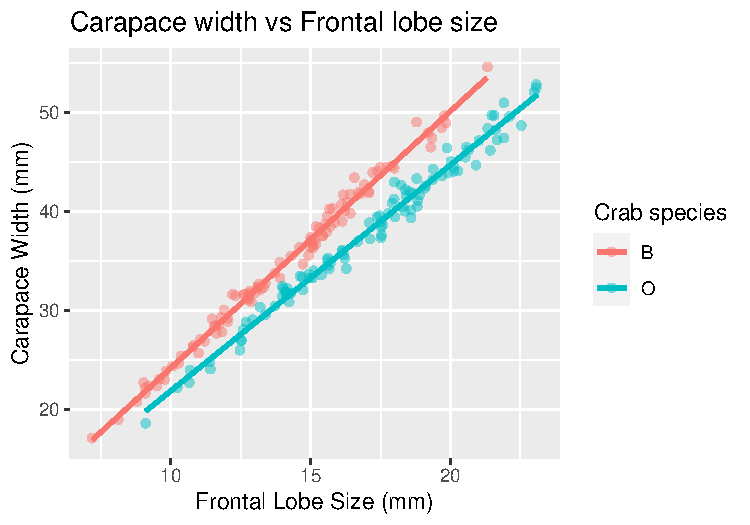
\includegraphics{Log_files/figure-latex/figure1-1} 

}

\caption{Spread of Front lobe size against Carapace width based on color}\label{fig:figure1}
\end{figure}

This plot plots the frontal lobe size against the carapace width of the
blue crabs as blue dots, and of the orange crabs as orange dots. It
shows that blue crabs on average have wider carapaces and shorter
frontal lobes, and that these attributes are somewhat correlated. This
could be a good indicator to determine the subspecies of the crab.
\newpage

\hypertarget{scatterplot-for-rear-width-against-carapace-length}{%
\subsubsection{Scatterplot for rear width against carapace
length}\label{scatterplot-for-rear-width-against-carapace-length}}

\begin{Shaded}
\begin{Highlighting}[]
\CommentTok{\#plot the Rear width against Carapace length}
\FunctionTok{ggplot}\NormalTok{() }\SpecialCharTok{+}
  \FunctionTok{geom\_point}\NormalTok{(}\AttributeTok{data =}\NormalTok{ myData[myData}\SpecialCharTok{$}\NormalTok{sp }\SpecialCharTok{==} \StringTok{"B"}\NormalTok{,], }\AttributeTok{mapping =} \FunctionTok{aes}\NormalTok{(}\AttributeTok{x =}\NormalTok{ RW, }\AttributeTok{y =}\NormalTok{ CL, }\AttributeTok{color =} \StringTok{\textquotesingle{}Blue\textquotesingle{}}\NormalTok{)) }\SpecialCharTok{+}
  \FunctionTok{geom\_point}\NormalTok{(}\AttributeTok{data =}\NormalTok{ myData[myData}\SpecialCharTok{$}\NormalTok{sp }\SpecialCharTok{==} \StringTok{"O"}\NormalTok{,], }\AttributeTok{mapping =} \FunctionTok{aes}\NormalTok{(}\AttributeTok{x =}\NormalTok{ RW, }\AttributeTok{y =}\NormalTok{ CL, }\AttributeTok{color =} \StringTok{\textquotesingle{}Orange\textquotesingle{}}\NormalTok{)) }\SpecialCharTok{+}
  \FunctionTok{scale\_color\_manual}\NormalTok{(}\AttributeTok{values=}\FunctionTok{c}\NormalTok{(}\StringTok{"\#4444EE"}\NormalTok{, }\StringTok{"\#E69F00"}\NormalTok{)) }\SpecialCharTok{+}
  \FunctionTok{labs}\NormalTok{(}\AttributeTok{x =} \StringTok{"Rear width (mm)"}\NormalTok{, }\AttributeTok{y =} \StringTok{"Carapace length (mm)"}\NormalTok{, }\AttributeTok{title=}\StringTok{\textquotesingle{}Rear width against Carapace length\textquotesingle{}}\NormalTok{)}
\end{Highlighting}
\end{Shaded}

\begin{figure}[H]

{\centering 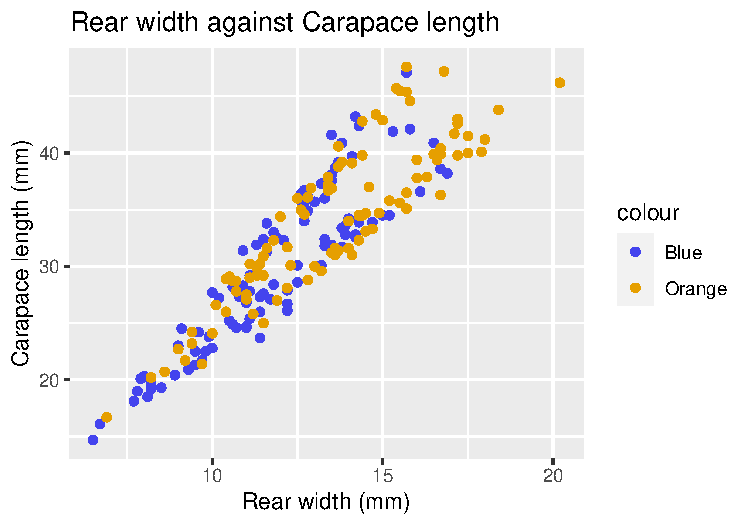
\includegraphics{Log_files/figure-latex/figure2-1} 

}

\caption{Spread of Rear width against Carapace length based on color}\label{fig:figure2}
\end{figure}

In this plot, the datapoints of the blue crabs are colored blue, and the
datapoints of the orange crabs colored orange again. This plot however,
does not show a clear difference between blue and orange crabs. Still
there are 2 separated groups, this means that these attributes are also
somewhat correlated and this could be investigated further. \newpage

\hypertarget{scatterplot-for-body-depth-against-carapace-width}{%
\subsubsection{Scatterplot for body depth against carapace
width}\label{scatterplot-for-body-depth-against-carapace-width}}

\begin{Shaded}
\begin{Highlighting}[]
\CommentTok{\#plot the Body depth against Carapace width}
\FunctionTok{ggplot}\NormalTok{() }\SpecialCharTok{+}
  \FunctionTok{geom\_point}\NormalTok{(}\AttributeTok{data =}\NormalTok{ myData[myData}\SpecialCharTok{$}\NormalTok{sp }\SpecialCharTok{==} \StringTok{"B"}\NormalTok{,], }\AttributeTok{mapping =} \FunctionTok{aes}\NormalTok{(}\AttributeTok{x =}\NormalTok{ BD, }\AttributeTok{y =}\NormalTok{ CW, }\AttributeTok{color =} \StringTok{\textquotesingle{}Blue\textquotesingle{}}\NormalTok{)) }\SpecialCharTok{+}
  \FunctionTok{geom\_point}\NormalTok{(}\AttributeTok{data =}\NormalTok{ myData[myData}\SpecialCharTok{$}\NormalTok{sp }\SpecialCharTok{==} \StringTok{"O"}\NormalTok{,], }\AttributeTok{mapping =} \FunctionTok{aes}\NormalTok{(}\AttributeTok{x =}\NormalTok{ BD, }\AttributeTok{y =}\NormalTok{ CW, }\AttributeTok{color =} \StringTok{\textquotesingle{}Orange\textquotesingle{}}\NormalTok{)) }\SpecialCharTok{+}
  \FunctionTok{scale\_color\_manual}\NormalTok{(}\AttributeTok{values=}\FunctionTok{c}\NormalTok{(}\StringTok{"\#4444EE"}\NormalTok{, }\StringTok{"\#E69F00"}\NormalTok{)) }\SpecialCharTok{+}
  \FunctionTok{labs}\NormalTok{(}\AttributeTok{x =} \StringTok{"Body depth (mm)"}\NormalTok{, }\AttributeTok{y =} \StringTok{"Carapace width (mm)"}\NormalTok{, }\AttributeTok{title=}\StringTok{\textquotesingle{}Body depth against Carapace width\textquotesingle{}}\NormalTok{)}
\end{Highlighting}
\end{Shaded}

\begin{figure}[H]

{\centering 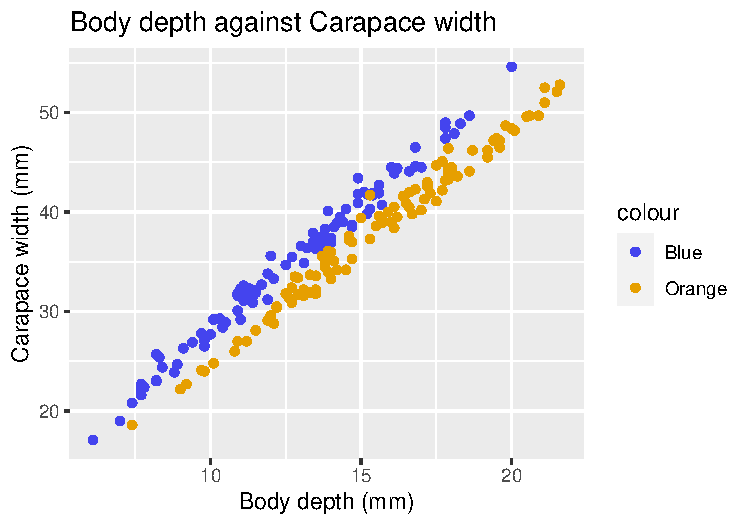
\includegraphics{Log_files/figure-latex/figure3-1} 

}

\caption{Spread of Body depth against Carapace width based on color}\label{fig:figure3}
\end{figure}

In this plot, again the datapoints were colored to represent the color
of the crab. This plot also shows that blue crabs on average have wider
carapaces, but that orange crabs tend to have deeper bodies, and that
these attributes are somewhat correlated. This could also be a good
indicator to determine the subspecies of the crab, though its less clear
than figure 1. \newpage

\hypertarget{scatterplot-for-rear-width-against-carapace-length-1}{%
\subsubsection{Scatterplot for rear width against carapace
length}\label{scatterplot-for-rear-width-against-carapace-length-1}}

\begin{Shaded}
\begin{Highlighting}[]
\CommentTok{\# plot the rear width against the carapace length based on gender}
\FunctionTok{ggplot}\NormalTok{() }\SpecialCharTok{+}
  \FunctionTok{geom\_point}\NormalTok{(}\AttributeTok{data =}\NormalTok{ myData[myData}\SpecialCharTok{$}\NormalTok{sex }\SpecialCharTok{==} \StringTok{"F"}\NormalTok{,], }\AttributeTok{mapping =} \FunctionTok{aes}\NormalTok{(}\AttributeTok{x =}\NormalTok{ RW, }\AttributeTok{y =}\NormalTok{ CL, }\AttributeTok{color =} \StringTok{\textquotesingle{}Female\textquotesingle{}}\NormalTok{)) }\SpecialCharTok{+}
  \FunctionTok{geom\_point}\NormalTok{(}\AttributeTok{data =}\NormalTok{ myData[myData}\SpecialCharTok{$}\NormalTok{sex }\SpecialCharTok{==} \StringTok{"M"}\NormalTok{,], }\AttributeTok{mapping =} \FunctionTok{aes}\NormalTok{(}\AttributeTok{x =}\NormalTok{ RW, }\AttributeTok{y =}\NormalTok{ CL, }\AttributeTok{color =} \StringTok{\textquotesingle{}Male\textquotesingle{}}\NormalTok{)) }\SpecialCharTok{+}
  \FunctionTok{scale\_color\_manual}\NormalTok{(}\AttributeTok{values=}\FunctionTok{c}\NormalTok{(}\StringTok{"\#EE4444"}\NormalTok{, }\StringTok{"\#4444EE"}\NormalTok{)) }\SpecialCharTok{+}
  \FunctionTok{labs}\NormalTok{(}\AttributeTok{x =} \StringTok{"Rear width (mm)"}\NormalTok{, }\AttributeTok{y =} \StringTok{"Carapace length (mm)"}\NormalTok{, }\AttributeTok{title=}\StringTok{\textquotesingle{}Carapace length against Rear width based on gender\textquotesingle{}}\NormalTok{)}
\end{Highlighting}
\end{Shaded}

\begin{figure}[H]

{\centering 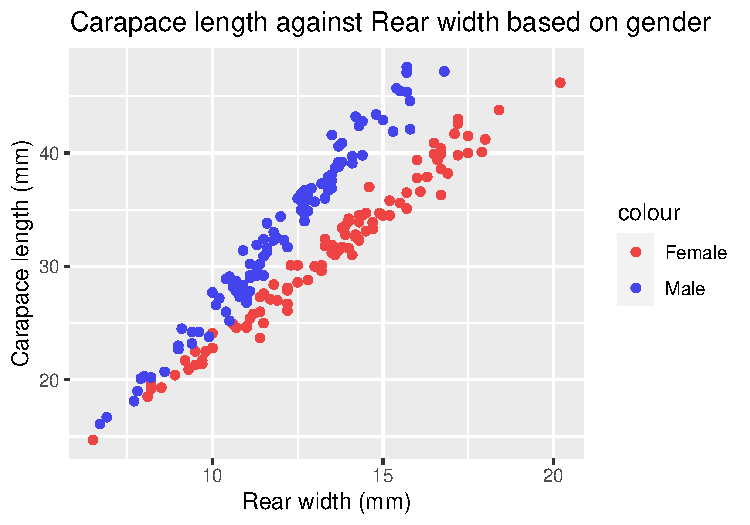
\includegraphics{Log_files/figure-latex/figure4-1} 

}

\caption{Spread of Carapace length against Rear width based on gender}\label{fig:figure4}
\end{figure}

This plot was created to further investigate the two groups of figure 2.
Instead of coloring the datapoints blue and orange based on the color of
the crab, the datapoints in this plot were colored according to the
gender. Blue for male crabs and red for female crabs. As shown in figure
4, it is indeed two groups of the genders of the crabs. This means that
the males have longer carapaces than the females. \newpage

\hypertarget{boxplot-of-carapace-length-for-the-genders}{%
\subsubsection{Boxplot of carapace length for the
genders}\label{boxplot-of-carapace-length-for-the-genders}}

\begin{Shaded}
\begin{Highlighting}[]
\CommentTok{\# sepperate the orange and blue crabs}
\NormalTok{orangecrabs }\OtherTok{\textless{}{-}}\NormalTok{ myData[myData}\SpecialCharTok{$}\NormalTok{sp }\SpecialCharTok{==} \StringTok{"O"}\NormalTok{,]}
\NormalTok{bluecrabs }\OtherTok{\textless{}{-}}\NormalTok{ myData[myData}\SpecialCharTok{$}\NormalTok{sp }\SpecialCharTok{==} \StringTok{"B"}\NormalTok{,]}

\FunctionTok{ggplot}\NormalTok{(}\AttributeTok{data=}\NormalTok{myData, }\AttributeTok{mapping =} \FunctionTok{aes}\NormalTok{(}\AttributeTok{x=}\NormalTok{sex, }\AttributeTok{y=}\NormalTok{CL)) }\SpecialCharTok{+}
  \FunctionTok{geom\_boxplot}\NormalTok{(}\AttributeTok{notch=}\ConstantTok{TRUE}\NormalTok{, }\AttributeTok{fill=}\FunctionTok{c}\NormalTok{(}\StringTok{"\#EE4444"}\NormalTok{, }\StringTok{"\#4444EE"}\NormalTok{)) }\SpecialCharTok{+}
  \FunctionTok{labs}\NormalTok{(}\AttributeTok{x =} \StringTok{"Gender"}\NormalTok{, }\AttributeTok{y =} \StringTok{\textquotesingle{}Carapace length (mm)\textquotesingle{}}\NormalTok{, }\AttributeTok{title=}\StringTok{\textquotesingle{}All crabs\textquotesingle{}}\NormalTok{)}
\end{Highlighting}
\end{Shaded}

\begin{figure}[H]

{\centering 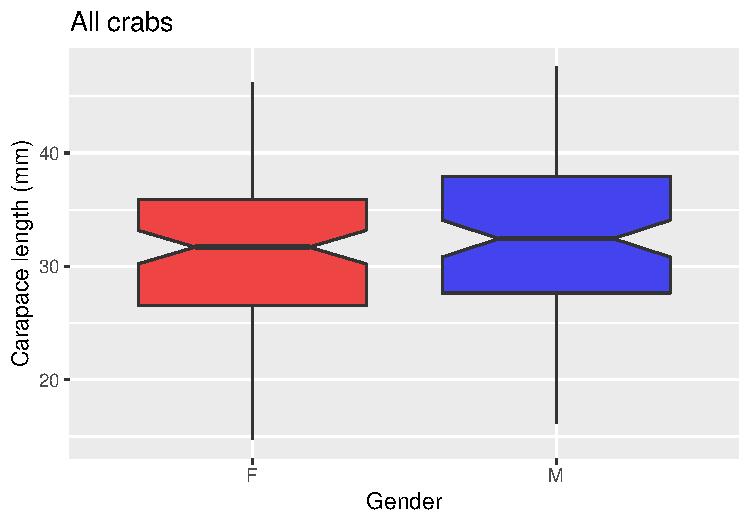
\includegraphics{Log_files/figure-latex/figure5-1} 

}

\caption{Distribution of Carapace length for all male and female crabs}\label{fig:figure5}
\end{figure}

This plot was created to further investigate the difference in carapace
length for the genders instead of the color of the crab. This plot does
not show a big difference between male and female crabs. The female
crabs have a slightly shorter carapace, but it does not seem
significant. This could be investigated further, but is not much
connected to the research question. \newpage

\hypertarget{boxplots-of-the-carapace-length-for-each-gender}{%
\subsubsection{Boxplots of the carapace length for each
gender}\label{boxplots-of-the-carapace-length-for-each-gender}}

\begin{Shaded}
\begin{Highlighting}[]
\FunctionTok{require}\NormalTok{(gridExtra)}

\NormalTok{ocrabs }\OtherTok{\textless{}{-}} \FunctionTok{ggplot}\NormalTok{(}\AttributeTok{data=}\NormalTok{orangecrabs, }\AttributeTok{mapping =} \FunctionTok{aes}\NormalTok{(}\AttributeTok{x=}\NormalTok{sex, }\AttributeTok{y=}\NormalTok{CL)) }\SpecialCharTok{+}
  \FunctionTok{geom\_boxplot}\NormalTok{(}\AttributeTok{notch=}\ConstantTok{TRUE}\NormalTok{, }\AttributeTok{fill=}\FunctionTok{c}\NormalTok{(}\StringTok{"\#EE4444"}\NormalTok{, }\StringTok{"\#4444EE"}\NormalTok{)) }\SpecialCharTok{+}
  \FunctionTok{labs}\NormalTok{(}\AttributeTok{x =} \StringTok{"Gender"}\NormalTok{, }\AttributeTok{y =} \StringTok{\textquotesingle{}Carapace length (mm)\textquotesingle{}}\NormalTok{, }\AttributeTok{title=}\StringTok{\textquotesingle{}Orange crabs\textquotesingle{}}\NormalTok{)}

\NormalTok{bcrabs }\OtherTok{\textless{}{-}} \FunctionTok{ggplot}\NormalTok{(}\AttributeTok{data=}\NormalTok{bluecrabs, }\AttributeTok{mapping =} \FunctionTok{aes}\NormalTok{(}\AttributeTok{x=}\NormalTok{sex, }\AttributeTok{y=}\NormalTok{CL)) }\SpecialCharTok{+}
  \FunctionTok{geom\_boxplot}\NormalTok{(}\AttributeTok{notch=}\ConstantTok{TRUE}\NormalTok{, }\AttributeTok{fill=}\FunctionTok{c}\NormalTok{(}\StringTok{"\#EE4444"}\NormalTok{, }\StringTok{"\#4444EE"}\NormalTok{)) }\SpecialCharTok{+}
  \FunctionTok{labs}\NormalTok{(}\AttributeTok{x =} \StringTok{"Gender"}\NormalTok{, }\AttributeTok{y =} \StringTok{\textquotesingle{}Carapace length (mm)\textquotesingle{}}\NormalTok{, }\AttributeTok{title=}\StringTok{\textquotesingle{}Blue crabs\textquotesingle{}}\NormalTok{)}

\FunctionTok{grid.arrange}\NormalTok{(bcrabs, ocrabs, }\AttributeTok{ncol=}\DecValTok{2}\NormalTok{)}
\end{Highlighting}
\end{Shaded}

\begin{figure}[H]

{\centering 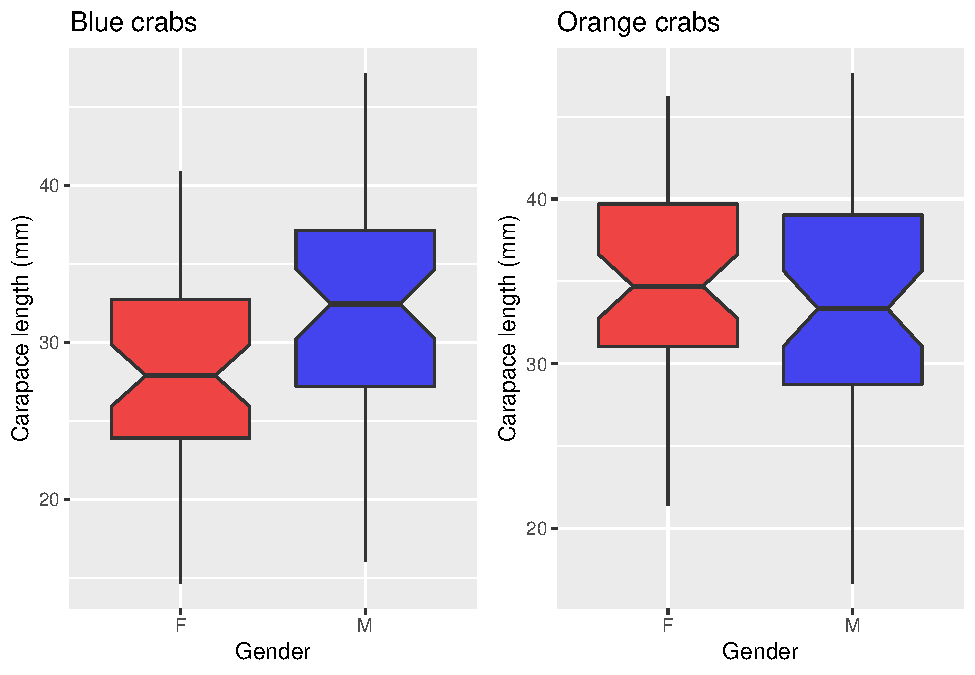
\includegraphics{Log_files/figure-latex/figure6-1} 

}

\caption{Distribution of Carapace length for the orange and the blue male and female crabs}\label{fig:figure6}
\end{figure}

To investigate further upon the difference in carapace length based on
the gender, these two boxplots were created to show the difference in
carapace length for each gender for each color. Figure 6 shows a small
difference in the length of the carapace between male and female orange
crabs. It shows that the male crabs have on average a shorter carapace,
but the difference is not that big. Figure 7 shows a bigger difference
in the length of the carapace between male and female blue crabs. Here,
the difference in means does seem significant. As shown in figure 7, it
is mainly the blue crabs that have a significant difference in carapace
length between genders. It shows that the male crabs have longer
carapace lengths on average. In figure 6 its clear that the male orange
crabs have shorter carapace lengths on average compared to the females.
\newpage

\hypertarget{pca-plot}{%
\subsubsection{PCA plot}\label{pca-plot}}

\begin{Shaded}
\begin{Highlighting}[]
\NormalTok{res.pca }\OtherTok{\textless{}{-}} \FunctionTok{PCA}\NormalTok{(myData[}\DecValTok{4}\SpecialCharTok{:}\FunctionTok{ncol}\NormalTok{(myData)], }\AttributeTok{ncp =} \DecValTok{5}\NormalTok{, }\AttributeTok{graph =} \ConstantTok{FALSE}\NormalTok{)}

\FunctionTok{fviz\_pca\_var}\NormalTok{(res.pca, }\AttributeTok{col.var =} \StringTok{"cos2"}\NormalTok{,}
             \AttributeTok{gradient.cols =} \FunctionTok{c}\NormalTok{(}\StringTok{"\#00AFBB"}\NormalTok{, }\StringTok{"\#E7B800"}\NormalTok{, }\StringTok{"\#FC4E07"}\NormalTok{), }
             \AttributeTok{repel =} \ConstantTok{TRUE}\NormalTok{)}
\end{Highlighting}
\end{Shaded}

\begin{center}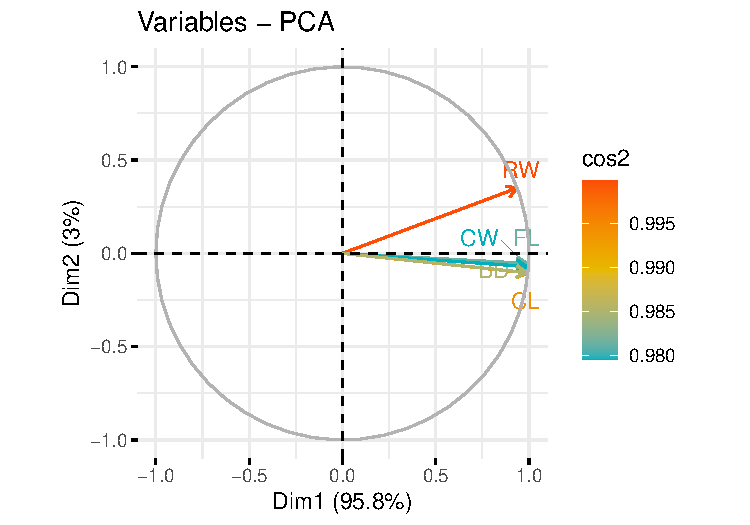
\includegraphics{Log_files/figure-latex/pca-1} \end{center}

This PCA plot was created to show the correlation between all variables.
This PCA plot shows that the variables are highly correlated. The least
correlated variable is the Rear width. This vector has the largest angle
with the Carapace length, the same two variables that were used to
discover the difference in carapace length distribution between the
genders.

\newpage

\hypertarget{machine-learning}{%
\subsection{Machine learning}\label{machine-learning}}

\hypertarget{cleaning}{%
\subsubsection{cleaning}\label{cleaning}}

Before machine learning can be used, the data must first be cleaned. In
its current form, the data is not ready for machine learning. Because of
the id column, some of the machine learning algorithms overfit their
model by using this column. So this column should be removed first. The
species columns was also moved to the last column so it would be used as
the class attribute.

\begin{Shaded}
\begin{Highlighting}[]
\NormalTok{clean\_data }\OtherTok{\textless{}{-}}\NormalTok{ myData[,}\FunctionTok{c}\NormalTok{(}\DecValTok{2}\NormalTok{,}\DecValTok{4}\SpecialCharTok{:}\FunctionTok{ncol}\NormalTok{(myData), }\DecValTok{1}\NormalTok{)]}
\FunctionTok{write.csv}\NormalTok{(clean\_data, }\StringTok{"datafiles/cleanedData.csv"}\NormalTok{, }\AttributeTok{row.names =}\NormalTok{ F, }\AttributeTok{col.names =}\NormalTok{ F)}
\end{Highlighting}
\end{Shaded}

\hypertarget{weka}{%
\subsubsection{WEKA}\label{weka}}

To find out what machine learning algorithm is the best for predicting
the species of crab, multiple algorithms were tested. These algorithms
are ZeroR, OneR, Simple logistic, Naive bayes, Random forest, J48, SMO
and K-nearest neighbor. These algorithms were tested using 10 fold
cross-validation. The highest quality metric for this dataset is the
accuracy, since it does not matter whether a blue crab is predicted to
be orange, or an orange crab to be blue. The software used to calculate
the accuracy is weka. After the classification, the accuracy of these
algorithms was saved in a csv file, and are shown in this barplot below.

\begin{Shaded}
\begin{Highlighting}[]
\NormalTok{algorithms }\OtherTok{\textless{}{-}} \FunctionTok{read.csv}\NormalTok{(}\StringTok{"datafiles/ml.csv"}\NormalTok{)}
\FunctionTok{ggplot}\NormalTok{(}\AttributeTok{data=}\FunctionTok{as.data.frame}\NormalTok{(algorithms), }\AttributeTok{mapping =} \FunctionTok{aes}\NormalTok{(}\AttributeTok{x=}\FunctionTok{reorder}\NormalTok{(Algorithm,}\SpecialCharTok{+}\NormalTok{Accuracy), }\AttributeTok{y=}\NormalTok{Accuracy)) }\SpecialCharTok{+}
  \FunctionTok{geom\_bar}\NormalTok{(}\AttributeTok{stat =} \StringTok{\textquotesingle{}identity\textquotesingle{}}\NormalTok{) }\SpecialCharTok{+}
  \FunctionTok{labs}\NormalTok{(}\AttributeTok{x =} \StringTok{"Algorithm"}\NormalTok{, }\AttributeTok{y =} \StringTok{\textquotesingle{}Accuracy (\%)\textquotesingle{}}\NormalTok{, }\AttributeTok{title=}\StringTok{\textquotesingle{}Accuracy of algorithms\textquotesingle{}}\NormalTok{)}
\end{Highlighting}
\end{Shaded}

\begin{figure}[H]

{\centering 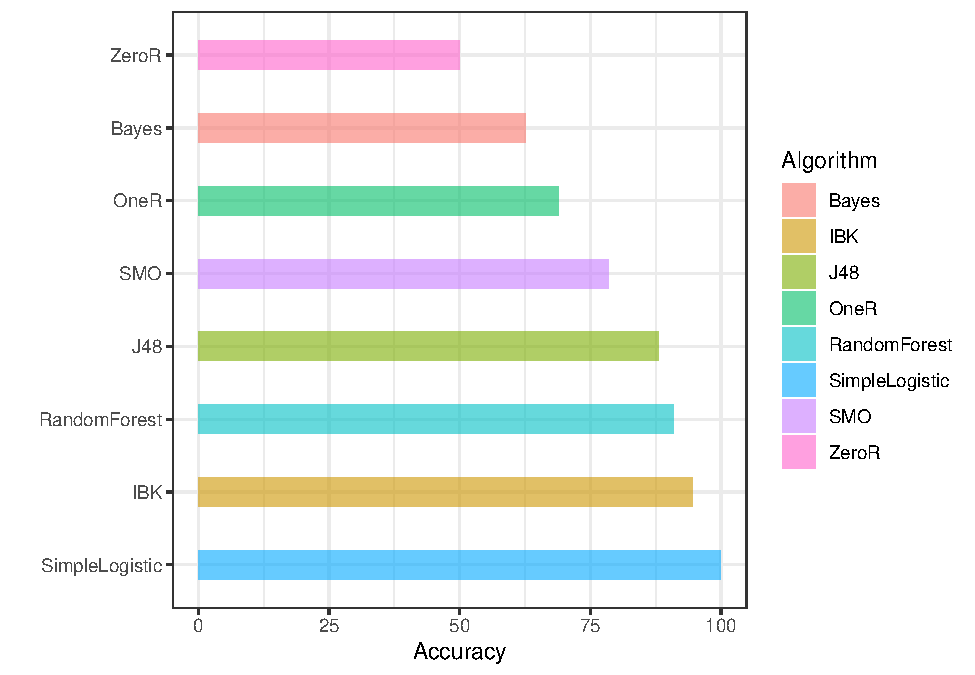
\includegraphics{Log_files/figure-latex/ml-1} 

}

\caption{The accuracy of the machine learning algorithms ordered from low to high.}\label{fig:ml}
\end{figure}

This plot shows a few interesting things, most notably the 100\%
accuracy of Simple logistic. The output in weka of the classification
using Simple logistic with 10 fold cross-validation shows a model for
each species. The model for the blue crabs shows 1.03 + {[}FL{]} * -0.6
+ {[}CW{]} * 0.31 + {[}BD{]} * -0.22. The model for the orange crabs
shows -1.03 + {[}FL{]} * 0.6 + {[}CW{]} * -0.31 + {[}BD{]} * 0.22. The
values in the model of the orange crabs are the values of the model of
the blue crabs times -1. The metrics used in the models are Front lobe
size, Carapace width and Body depth. The barplot also shows an exact
50\% accuracy for the ZeroR algorithm. This is expected since the data
has the same amount of blue crabs as orange crabs.

Using the output from the simple logistic algorithm, the following roc
curve can be made.

\begin{center}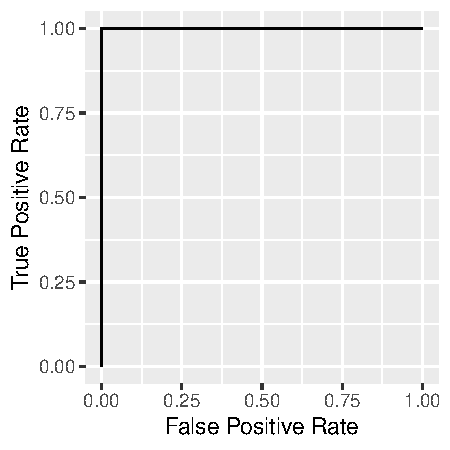
\includegraphics{Log_files/figure-latex/roc-1} \end{center}

The curve is of course two straight lines because the accuracy is 100\%.

\newpage

\hypertarget{discussion-and-future-research}{%
\subsection{Discussion and future
research}\label{discussion-and-future-research}}

The goal was to get the dataset ready for machine learning. The data was
analyzed and cleaned to make so it is ready to be used in machine
learning algorithms. The data does not contain many outliers. The data
points seem easy to classify since most plots show clear groups of blue
and orange crabs. As shown in figure 4, the gender of the crab could
also be a good attribute to help predict the species of crab. The data
also had to be cleaned. This was done by removing the index column,
since this column can not be used to help determine the species of crab.
It might also be a problematic attribute for some machine learning
algorithms. Then, the species column was moved to the last column, so
the machine learning algorithms will use this column as the class index.

Future research can be used to show more correlation between other
measurements. It can be researched whether or not the gender of the crab
could be predicted using these morphological measurements. Machine
learning use could also be improved by expanding the dataset, or getting
different amounts of blue or orange crabs, with different amounts of
male and female crabs.

\newpage

\end{document}
